\section{Background and Related Work}
\label{sec:related}

% Refer to past work in AUV autonomy as well as robotic autonomy in
% general. This is general purpose and should be a good literature survey
% for robotics and AI.

A distinct problem in Marine Robotics has been the use of the
overloaded term 'autonomy'. Not only does the notion transcend
different disciplines within engineering in this domain (e.g. the
Control Engineering community sees it distinctively from those in AI)
but users of marine platforms in oceanography as well as in maritime
defense conflate the methodology of use (tethered vs. untethered) with
their control. In this chapter, our notion of 'autonomy' refers not
only to the notion of dealing with the \emph{sense, plan and act}
paradigm in robotics, but also the need to perform \emph{computational
  search} between different action outcomes, an idea central to the
field of AI. Consequently, our literature survey here is targeted
towards a more focused and (to this chapter) relevant part of the
field of computation.

With few exceptions, most AUV control systems have been variations of
reactive approaches.  Typically, waypoint-based pre-defined mission
designs are uploaded to the AUV; specialized code fragments called
\emph{behaviors} are designed for the specific mission and a choice of
behaviors for the mission are used on the computational stack
\cite{bellingham94}. Swapping in and out of these behaviors using
conditionals or cleverer and quantitative approaches such as
\cite{Benjamin:2004} forms the basis for adaptation and safety in the
vehicle. Where such swapping does not aid adaptation, individual
behaviors are tweaked to generate some measure of responsiveness to
the surrounding environment \cite{yanwu08} to generate interesting
observations for oceanographers, yet technically naive in terms of
scalability and systematicity. \cite{Benjamin2006} is clear about the
\kcomment{extent} of adaptation in stating:

{\footnotesize
  \begin{quote}
\small \emph{The primary difficulty often associated with behavior-based control
concerns action selection - namely how to ensure the chosen action
really is in the best overall interest of the robot or vehicle.}
\end{quote}
} 

Such techniques have proved their mettle in the first round of use of
AUVs; they've provided operators a simple way to handle control
complexity of the vehicle while returned data at far higher resolution
than would have been possible using traditional ship-based methods and
at substantially reduced amortized costs of platform operation and
ownership over multiple years. AUV operators and clients for their
data products have reasons to be well satisfied with results thus
far. However, as hardware and more cost-effective sensors become more
robust to the environment and as mission durations increase (as
demonstrated by glider experiments such as \cite{rucool11}), sustained
presence in the ocean requires the ability to deal with off-nominal
conditions, that balances the needs of high-level mission management,
low-level navigation, instrument control and detection of unstructured
and poorly understood phenomena. Earlier reactive methods are unable
to perform such a balancing act without skewering the foundations of
the software development methodology leading to code bloat or worse.
\cite{carreras06} provides a good overview of AUV control
architectures essentially based on reactive control methods.

Deliberative techniques for robotic control on the other hand
contrast in providing a distinct set of advantages:

\begin{enumerate}

\item action selection is driven axiomatically based on a systematic
  assessment of a range of causal conditions. An action is selected
  for instantiation only when there is causal support in the form of a
  constraint in a deterministic model of the vehicle's operation.

\item the system is goal directed which forms an objective towards
  which the system is expecting to converge providing a foci in action
  selection.

\item scaling to different (computational) problem size is dependent
  on incremental model building rather than being concerned about
  nuanced interactions between behaviors.

\item systematic software engineering methodologies such as spiral
  development \cite{boehm86} can further be used for scaling up the
  task as demonstrated by \cite{DS1report}.

\item when interactions between actions and/or behavior fragments do
  (and must) occur there are explicit constraints encoded in the model
  that must be computationally satisfied contrasting with carefully
  crafted strategies to instantiate behaviors on a stack. Such
  explicit recording of constraints in the model in turn aids
  long-term software maintenance and sustaining engineering.

\end{enumerate}

\begin{figure}[!t]
 \centering
 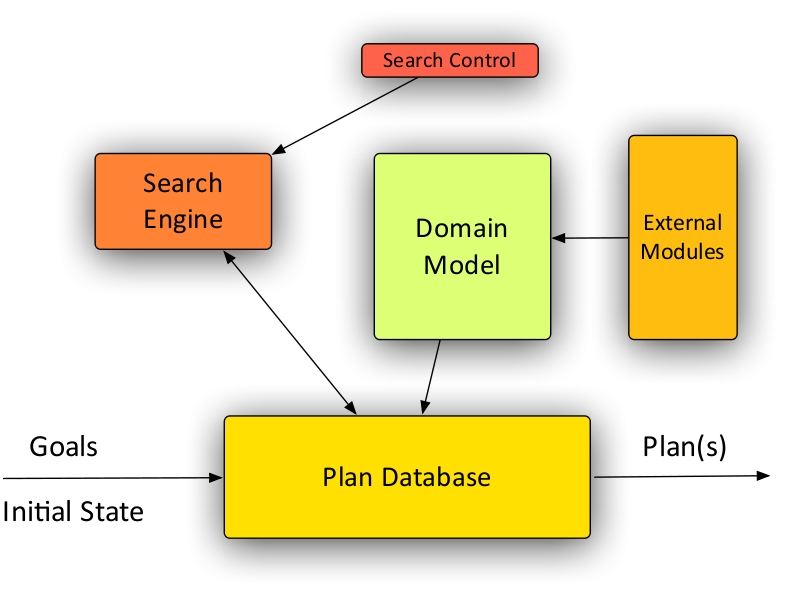
\includegraphics[scale=2]{figs/planner-arch.jpeg}
 \caption{\small A general architectural block diagram for an AI based
   Planner.}
 \label{fig:planner}
\end{figure}

Traditionally generalized planning has been considered computationally
intensive (the general planning problem can be worse than NP-complete
\cite{ghallab04}). A major reason for this belief had to do with the
role of the planner (which was assumed to be generative) and its place
in the architecture (infrequently called to re-plan the \emph{entire}
mission in off-nominal conditions) within a \emph{sense-plan-act}
paradigm. This can limit the reactivity of a robot especially when the
environment could change at a rate faster than the planner can plan.

The architecture of a typical AI planner is along the lines of
Fig. \ref{fig:planner}. Given a \emph{domain model} which encodes the
platform constraints in a higher-level language, an \emph{initial
  state}, a high-level objective or end \emph{goal}, the \emph{plan
  database} (or \texttt{plandb}) is where all assertions are tracked
and maintained. Theorem proving in the form of satisfaction of axioms
embodied in the domain model occurs within the \texttt{plandb}. It is
the job of the \emph{search engine} to provide the inferential
mechanism for state space exploration potentially aided by heuristics
encoded for \emph{search control}. In some complex domains
\cite{mus98} \emph{external modules} can provide additional domain
expertise which can augment the model. The end result is plan
formulation using a multitude of approaches either using forward or
backward search or using more generalized \emph{partial order} methods
\cite{ghallab04}.


There are costs associated with such inference based control which are
not inconsequential. Foremost among them is the steep learning curve
that comes with the design of the domain model. With limited support
tools necessary for knowledge capture and design of the constraints
often in stylized higher-level languages (see \cite{NDDL} for an
example), it requires the modeler to think in alternative ways to do
problem solving. More importantly it is often necessary for the
modeler to be exposed to the internal representation of the planner
and how it performs search. The level of expertise is often well above
what would be expected of a typical well-rounded Computer Science
graduate student. Yet in our experience, the cost of model design in
such systems, is well balanced against the cost of re-engineering new
mission scripts for new deployment in more ``classical'' script-based
controllers.

However this is mild criticism given the end benefits and the
scientific and engineering goals associated with adaptive and
persistent observation for marine robots whether for civil or military
applications. Given the general problem-solving nature of such
deliberative systems, there is also a substantial overall benefit for
the field of robotics.

\subsection{Evolution of AI-based Robotic Planning: A Necessary Digression}
\label{sec:related:robotplans}

Planning and plan execution are not new to the overall field of
robotics. Early motivation of building computational mechanisms for
decision making were intended to be deployed on robotic devices by
very definition. The seminal volume \cite{computersthought} very
clearly articulates how physical manifestation of robots could be
controlled by task planning and execution. The very first planner
\cite{green69} was an exercise in computational theorem proving with
early state space planners popularized by \texttt{STRIPS}
\cite{strips71} dominating the academic landscape. An early
demonstration of planning as a situated agent\footnote{\kcomment{By
    \emph{situated} we emphasize that an agent is embedded within a
    physical robot.}} was the highly influential \texttt{Shakey} the
robot \cite{shakey84}. Subsequent work driven largely by defense
funding in the United States sequestered the discipline in academic
labs principally applied for algorithmic development and if embedded
then in testing within the confines of \kcomment{structured} indoor
settings. The leap to applying them for real world problem solving is
relatively new and driven largely by NASA applications pioneered by
\cite{mus94,mus98, jonsson00, rajan00, chien05, bresina05}.

The dominant approach for building agent control systems utilize a
$3$-layered architecture (see \cite{gat98} for a well thought out
rationale \kcomment{and survey}), notable examples of which include
\texttt{IPEM} \cite{AmbrosIngerson88}, \texttt{ROGUE} \cite{Haigh98},
the LAAS Architecture \cite{alami:1998p820}, the Remote Agent
Experiment \texttt{RAX} \cite{mus98} and the Autonomous Spacecraft
Experiment \texttt{ASE} \cite{chien99} (see \cite{Knight01} for a
survey). 

Representationally, the first paper on managing time systematically
within AI Planning frameworks was \cite{dean87}; subsequent efforts by
Boddy and others \cite{Dean88,Boddy93} refined the notion of using a
temporal database and the conceptualization of temporal
intervals. Using these concepts Muscettola and others \cite{mus92,
  ghallab94, laborie95, cesta96} developed the notion of plan/schedule
envelopes using the notion of state variable instantiated
timelines. Simultaneously work by Dechter et.al \cite{dechter91}
resulted in efficient temporal constraint propagation which
systematically defined the notion of Simple Temporal Networks (STNs)
and path and arc consistency algorithms. This work neatly put together
earlier efforts by Mackworth and Freuder \cite{mackworth77, mack85}
and the Constraints community on propagation algorithms. In parallel
work in the UK, resulted in the design of \texttt{O-Plan}
\cite{currie91}, which leveraged the notion of constraints and metric
time, but within a Hierarchical Task Network (HTN) representation.
These efforts were soon after Vere’s paper on planning and time
\cite{vere83} which had a profound effect on the AI Planning
community. In particular the work of Muscettola \cite{mus94} was
embraced by NASA for telescope scheduling. Around the same time
period, researchers at LAAS came up with an architecture
\cite{alami:1998p820} which encapsulated the \texttt{IxTeT} planner
\cite{ghallab94} \kcomment{which dealt with time and resources}. It
featured advanced concepts for a temporal planner with the notion of
chronicles, plan recognition for partial plan fragments and early use
of systematic resource constraints. % Development on \texttt{IxTeT} has
% continued albeit at a slower pace with the contribution of various PhD
% students’ thesis.

\subsection{The Remote Agent Experiment and beyond}
\label{sec:rabeyond}

While \texttt{HSTS} \cite{mus94} was being implemented as a
ground-based planning tool for decision support for US based space
observations (EUVE and Cassini) \cite{mus95}, the opportunity to fly
onboard NASA’s New Millennium Deep Space $1$ came about. The design of
the Remote Agent Experiment \texttt{RAX} \cite{pell97, bernard98,
  pell98, mus98, DS1report, rajan00, jonsson00} was a direct off-shoot
of this effort where \texttt{HSTS} (written in LISP) was flown on
board and successfully commanded the spacecraft for a week in May
1999\footnote{This was the first (and to our knowledge only) software
  ever to been written in \texttt{LISP} to be flown in space.}. There
were a number of significant software engineering lessons learned with
the HSTS technology as \kcomment{implemented} for the RAX
\kcomment{experiment}:

\begin{enumerate}

\item Constraint-based representations were not only sufficient for
  plan synthesis, but valuable during debugging and development as a
  means of building a viable domain model.

\item Domain models when separated from the search engine as
  articulated by the model-based approach \cite{williams96a} ensured
  that sufficient effort would be targeted on human validation of the
  model building phase while ensuring that search engine stability
  across applications and domains resulted in lower cost to deploy.

\item Flexible temporal representation generating a range of plans as
  against a single plan, were robust for \kcomment{robotic} plan
  execution.

\item If planning and execution were disconnected (as in
  \texttt{RAX}), dispatchabilty \cite{mus98a} and controllability
  \cite{morris00} issues within temporal plans need be addressed. In
  \texttt{RAX}, a post-processing step was added to counter these
  effects. It was clear that execution needed access to the planners
  database and be able to propagate execution time constraints prior
  to command dispatching.

\end{enumerate}

It was with the demonstration of \texttt{RAX} $65$ Million miles in
outer space, that temporal reasoning using \kcomment{planning} methods
came to the forefront of AI Planning for situated agents. Lessons
learned from \texttt{RAX} led to the development of \texttt{IDEA}
\cite{mus02,mus04,Dias:2003ua,mus06} with the central theme of using
planners collectively for problem solving. Another critical theme was
iteratively and incremental plan repair of an anytime plan
\cite{Zaimag96} as proposed by \texttt{CASPER} \cite{chien00}.

This last lesson in particular had a lasting impact with the
observation that planning and execution are strongly
inter-related. This core concept was behind the next generation of the
Remote Agent, called \texttt{IDEA} (Intelligent Deployable Execution
Agents) where planning and execution were \emph{intertwined} within a
single domain model that spanned the most abstract (for high-level
planning) to the least (for diagnosis). \texttt{IDEA} \cite{mus02,
  mus04} agents were expected to interact to achieve plan formulation;
however there was no systematic framework for formally governing these
interactions. \texttt{IDEA} was also computationally heavy and
required substantial effort to customize for an application domain. It
did move to a retooled version of \texttt{HSTS}, called \eu
\cite{frank2003, barreiro09} while being ported to the C++ language.

While \texttt{IDEA} was being deployed as a coordinating executive for
earth analog rover deployments \cite{wetter05} a separate development
was undertaken to deploy the \eu planner for NASA’s Mars Exploration
Rovers (MER) mission. The \texttt{MAPGEN} (Mixed-initiative Activity
Plan GENerator) planner \cite{bresina03, aichang04, bresina05,
  bresina05a} as a decision support tool in the mixed-initiative mode;
\texttt{MAPGEN} continues to be used to this day to command the twin
rovers on the Red Planet. % While EUROPA2 was not
% designed as an embedded planner, NASA undertook a bottom-up
% re-implementation of the planner and substantially increased its
% performance. EUROPA2 was then released as open source to the AI
% community at large [Europa].

The Autonomous Sciencecraft Experiment (\texttt{ASE}) \cite{chien99,
  chien03} was another autonomy demonstration in space, this time for
a more observable vehicle, the EO-1 in Earth orbit. It encapsulated a
classical 3-layered architecture like \texttt{RAX}. Goals could not
only be sent by a ground segment, but also by an onboard science
driver which could encapsulate a range of Machine Learned feature
detectors which could trigger the planner. However \texttt{ASE} was
not an integrated system; the \texttt{CASPER} planner \cite{chien00}
would generate plans which were executed by a separate commercially
available rule-based system \cite{icl}. \texttt{CASPER} demonstrates
what is called as a \emph{continuous} paradigm for incremental
planning and iterative plan repair; this methodology takes the overall
mission plan and selectively plans \kcomment{for the} near-term at a
more detailed level.
% The system also uses iterative-repair as a way to fix
% plans; however this too is derived from a model of the mission and
% spacecraft constraints which allow simple reconfiguration modes
% towards replanning. 
Robust software engineering is also not an important aspect targeted
by \texttt{ASE} given the disparate models between the planner and the
rule-based executive. With such a system, real-time updates from the
environment could not be accommodated since the planner is a
monolithic computational environment. The rate of updates from the
science drivers is roughly \kcomment{on} the order of an earth orbit
on the EO-1 vehicle. As a result, the \texttt{ASE} is only an
incremental update on \texttt{RAX} and is not suitable for domains
where complex automated reasoning and asynchronous environmental
observations need to be factored in deliberation.

\texttt{TCA} \cite{simmons94} another framework for robot control and
has similar motivations to \texttt{RAX} and \texttt{ASE}. Reactivity
and deliberation are also key to \texttt{TCA} \kcomment{along with} a
systematic approach to development led to its design. However it
suffers from three key weaknesses. First it has a weaker
representational framework of Task Trees which require representation
of tasks within cleanly formulated hierarchies. Constraints between
branches within a task hierarchy are allowed; timing between leaves of
different trees is however not possible. Second, its temporal
framework does not deal with flexibility; time points are fixed and
while partial orders are possible, it does deal with execution time
uncertainty. Third, while \texttt{TCA} shares the notion of using
domain expertise of different planners, it does so thru a centralized
message passing mechanism. While this allows disparate code-bases to
talk to each other \kcomment{through} IPC (\kcomment{an} inter-process
communication or message passing mechanism), failure in the
centralized controller is tantamount to a system crash.

The \texttt{ReSSAC} project at ONERA \cite{teichteil07} \kcomment{is
  motivated by} controlling aerial UAV platforms for autonomous Search
and Rescue. Like \texttt{TCA}, the project uses a supervisor to
control planning and at the same time decouples the deliberation and
reactive components from the lower level functional layer. This
deliberate separation is partly because of the use of optimizing MDP’s
(Markov Decision Processes \cite{mdp93}) for planning which uses
probabilistic state transitions to determine the next course of action
based on perceived state. To overcome the typical problem of state
space explosion with MDPs, a local heuristic is used in order to
generate reachable goal states incrementally. This work however does
not deal with metric time \kcomment{and comes} with a modestly simple
model.

\texttt{CIRCA} \cite{musliner95} is an effort to bring decision making
for real-world problems with the augmented need to have
\emph{verifiable} controllers synthesized in-situ to ensure that
\kcomment{during state space exploration}, there are no erroneous
transitions to dangerous states by asynchronously generating
Test-Action-Pairs (TAPs).  These are annotated production rules
consisting of a set of tests (or preconditions) and a set of actions
to take if all the tests return true. TAPs are synthesized and
scheduled by \texttt{CIRCA} and provide a viable way to deal with a
dynamically changing world. \texttt{CIRCA} however differentiates
between reasoning about time and reasoning in real-time with the
implication that reasoning necessarily requires substantial
computation for state space exploration which negates the real-time
(and thus real-world) impact.

A key and early concern that dominated planning was that of
scalability.  The planning cycle in many approaches was \kcomment{(and
  is)} monolithic, often making fast reaction times impractical when
necessary for embedded robotic agents. Many of these systems (which
were $3$-layered) also utilized very different techniques for
specifying each layer in the architecture resulting in duplication of
effort and a diffusion of knowledge.  The work we highlight in this
chapter builds on the approach used by \texttt{IDEA} \cite{mus02,
  mus04} in utilizing a collection of controllers, each interleaving
planning and execution within a common framework. \texttt{IDEA}
however, provided no support for conflict resolution between
controllers, nor did it provide an efficient algorithm for integrating
current state within a controller, relying instead on a possibly
exponential planning algorithm. Efficient synchronization of state in
a partitioned structure is fundamental to making the approach
effective in practice.

Our system, \rxe, the focus of this chapter, is an agent control
structure formally defined as a composition of coordinated control
loops where sensing, planning and acting \kcomment{result} from
concurrent deliberating tasks within a formal framework.  \rx was
designed after carefully evaluating lessons learned from \texttt{IDEA}
to which it owes substantially the notion of partitioned problem
solving. Partitioning in \rx is systematic and methodologically
principled where we manage the information flow within the partitioned
structure to ensure consistency in order to direct the flow of goals
and observations in a timely manner. The resulting control structure
improves scalability since many details of each controller can be
encapsulated within a single control loop.  Furthermore, partitioning
increases robustness since controller failure can be localized to
enable graceful system degradation, making this an effective
\emph{divide-and-conquer} approach to \kcomment{solving} the overall
control problem.

A recent variation of the key idea of such controller composition
derived from \rx is \texttt{ROAR} \cite{degroote11} where lower-level
functional modules that control sensors are organized within a graph
hierarchy. One reason they cite such a structure \kcomment{as being}
essential is in dealing robustly to failure; an off-nominal condition
will allow rapid graph traversal to identify alternative ways in which
sensing tasks can be executed and therefore aiding \kcomment{platform}
responsiveness. % However,
% it is unclear whether to date this system actually deliberates and
% whether it is actually instantiated on a real platform for control.

% ``The whole partition must be accordingly reorganized: this kind of
% construction does not scale well over a large variety of missions,
% missing the objective of a versatile architecture for robots.''

%%% Local Variables: 
%%% mode: latex
%%% TeX-master: "setobook"
%%% End: 
